\documentclass{standalone}

\usepackage{times}
\usepackage{amsmath}
\usepackage{txfonts}

\usepackage{tikz}
\usetikzlibrary{intersections,positioning}

\usepackage{pgfplots}
\pgfplotsset{compat=1.12}

\begin{document}

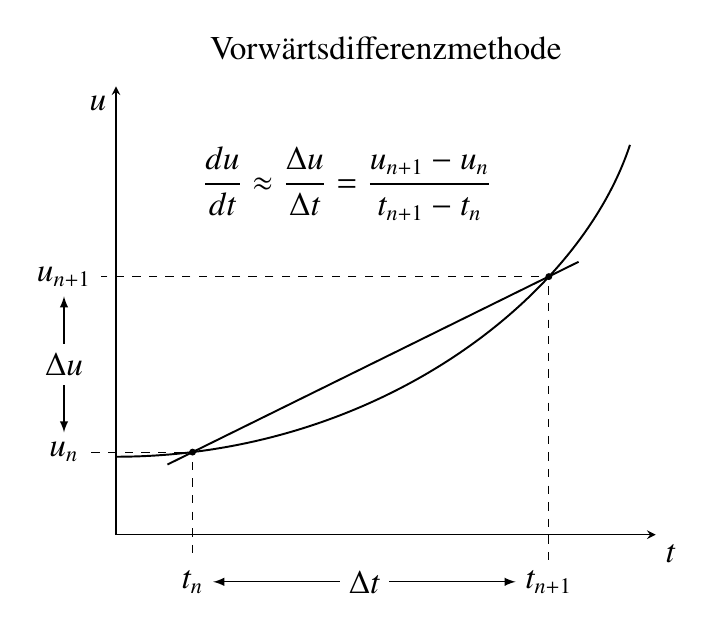
\begin{tikzpicture}[>=latex,scale=1,thick]

\begin{axis}[%
title={\large Vorwärtsdifferenzmethode},
ticks=none,
clip=false,
xlabel={\large $t$},
xmin=0,
xmax=10.5,
every axis x label/.style={at={(current axis.right of origin)},anchor=north west},
ylabel={\large $u$},
ymin=0,
ymax=5.75,
every axis y label/.style={at={(current axis.above origin)},anchor=north east},
axis x line=bottom,
axis y line = left]

%%%% Plot
\draw[name path global=CurveLine,line width=0.7pt] (0,1) .. controls (5,1) and (9,3) .. (10,5);

\addplot [name path global=StraightLine,line width=0.7pt] coordinates{(1,0.9) (9,3.5)};

\fill [name intersections={of=StraightLine and CurveLine, name=i, total=\t}][black] 
    \foreach \s in {1,...,\t}{(i-\s) circle (1.25pt)
        node (\s) {}};

%%%% Dashed lines and labels
\begin{scope}[dashed]

    \node[below=1.25cm of 1] (a) {\large $t_n$};
    \node (b) at (a -| 2) {\large $t_{n+1}$};

    \draw (1) -- (a);
    \draw (2) -- (b);

    \node[left=1.2cm of 1] (c) {\large $u_n$};
    \node (d) at (c |- 2) {\large $u_{n+1}$};

    \draw (1) -- (c);
    \draw (2) -- (d);

\end{scope}

\draw[<->] (a) --node[midway,fill=white]{\large $\Delta t$} (b);
\draw[<->] (c) --node[midway,fill=white]{\large $\Delta u$} (d);

\node at (4.5,4.5) {\large $\dfrac{du}{dt}\approx\dfrac{\Delta u}{\Delta t}=\dfrac{u_{n+1}-u_n}{t_{n+1}-t_n}$};

\end{axis}
\end{tikzpicture}

\end{document}
